\section*{Results}
The results are separated for registration and segmentation approaches. All were obtained with 20 training images and 10 test images. The results for each case are measured with the Dice score and the Hausdorff distance. They represented with boxplots to show the mean as well as the variability.

\subsection*{Registration}
Two registration methods have been implemented: affine (Aff) and non-rigid (NR). The first is easier to implement and faster to execute, the second one should match the atlas image better as more deformations are possible. The results for majority voting (MV) and machine learning (ML) are represented in figure \ref{fig:boxplotReg}.

\begin{figure}[h!]
	\centering
	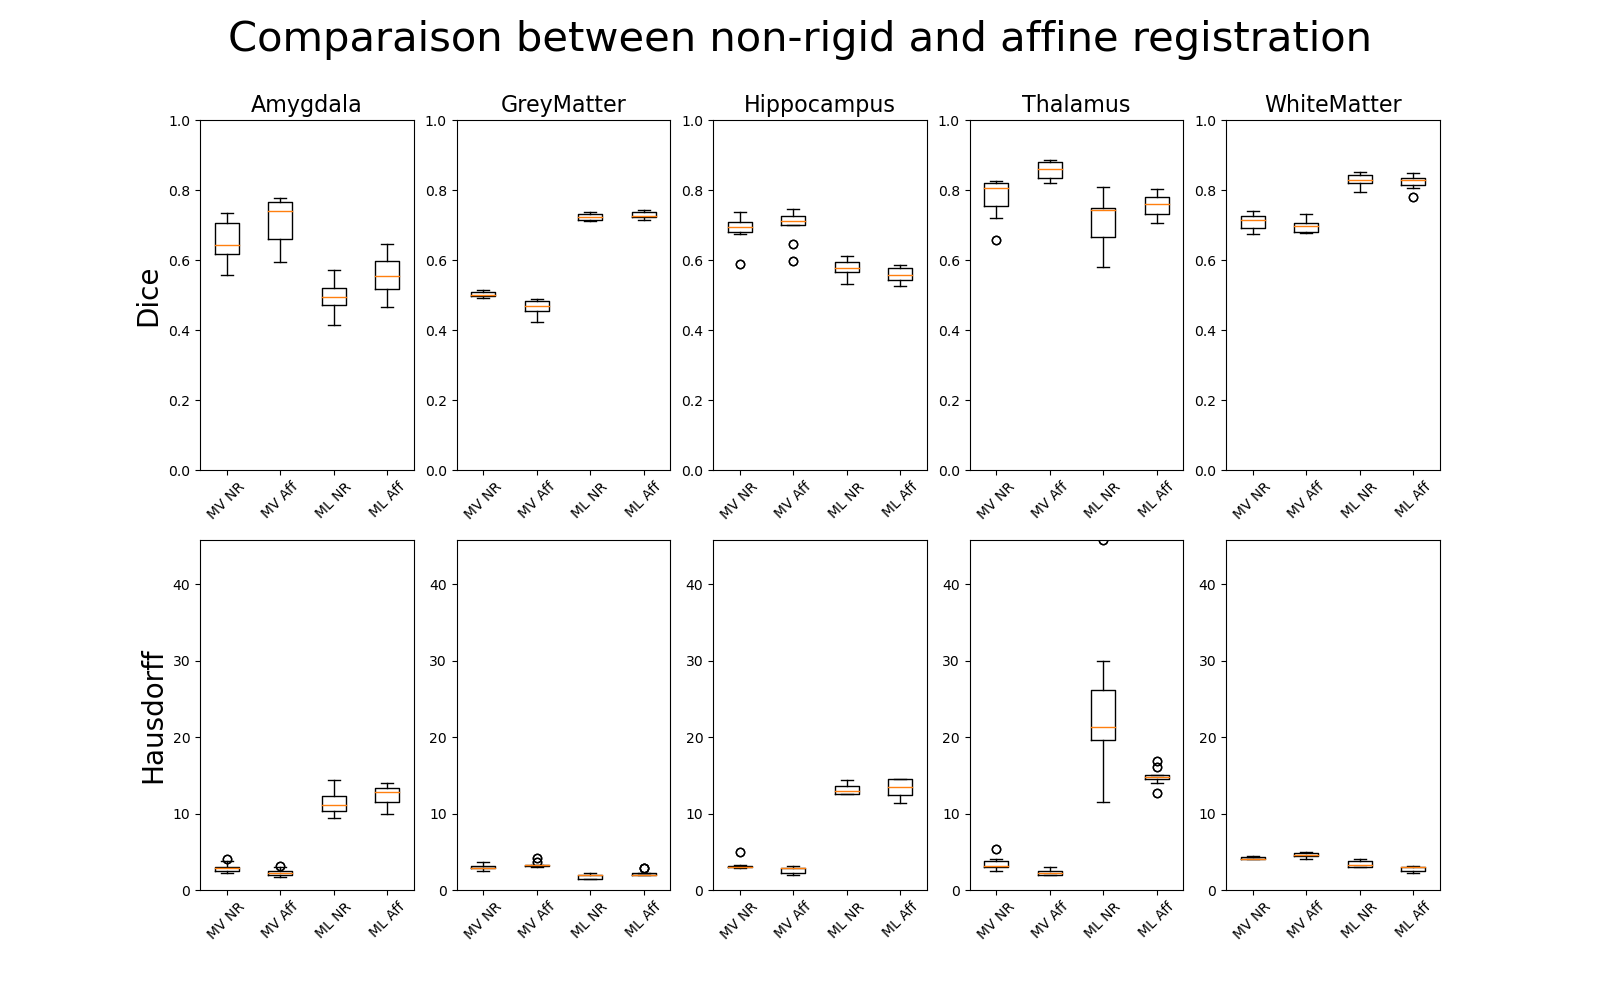
\includegraphics[width = .48 \textwidth]{img/boxplotComparisonNRAff}
	\caption{Dice and Hausdorff distance result for majority voting (MV) and machine learning (ML) segmentation preceded by non-rigid (NR) or affine (Aff) registration}
	\label{fig:boxplotReg}
\end{figure}

From the graphic, we can see no clear advantage of the non-rigid registration over the affine one. The difference is too small and has too much variability to choose one registration over the other one.

\subsection*{Segmentation}
Five segmentation methods have been implemented: majority voting (MV), global weighted (GW), local weighted (LW), shape based averaging (SBA) and machine learning (ML). All except the last one are atlas-based. The results with affine registration are represented in the figure \ref{fig:boxplotAff}.

\begin{figure}[h!]
	\centering
	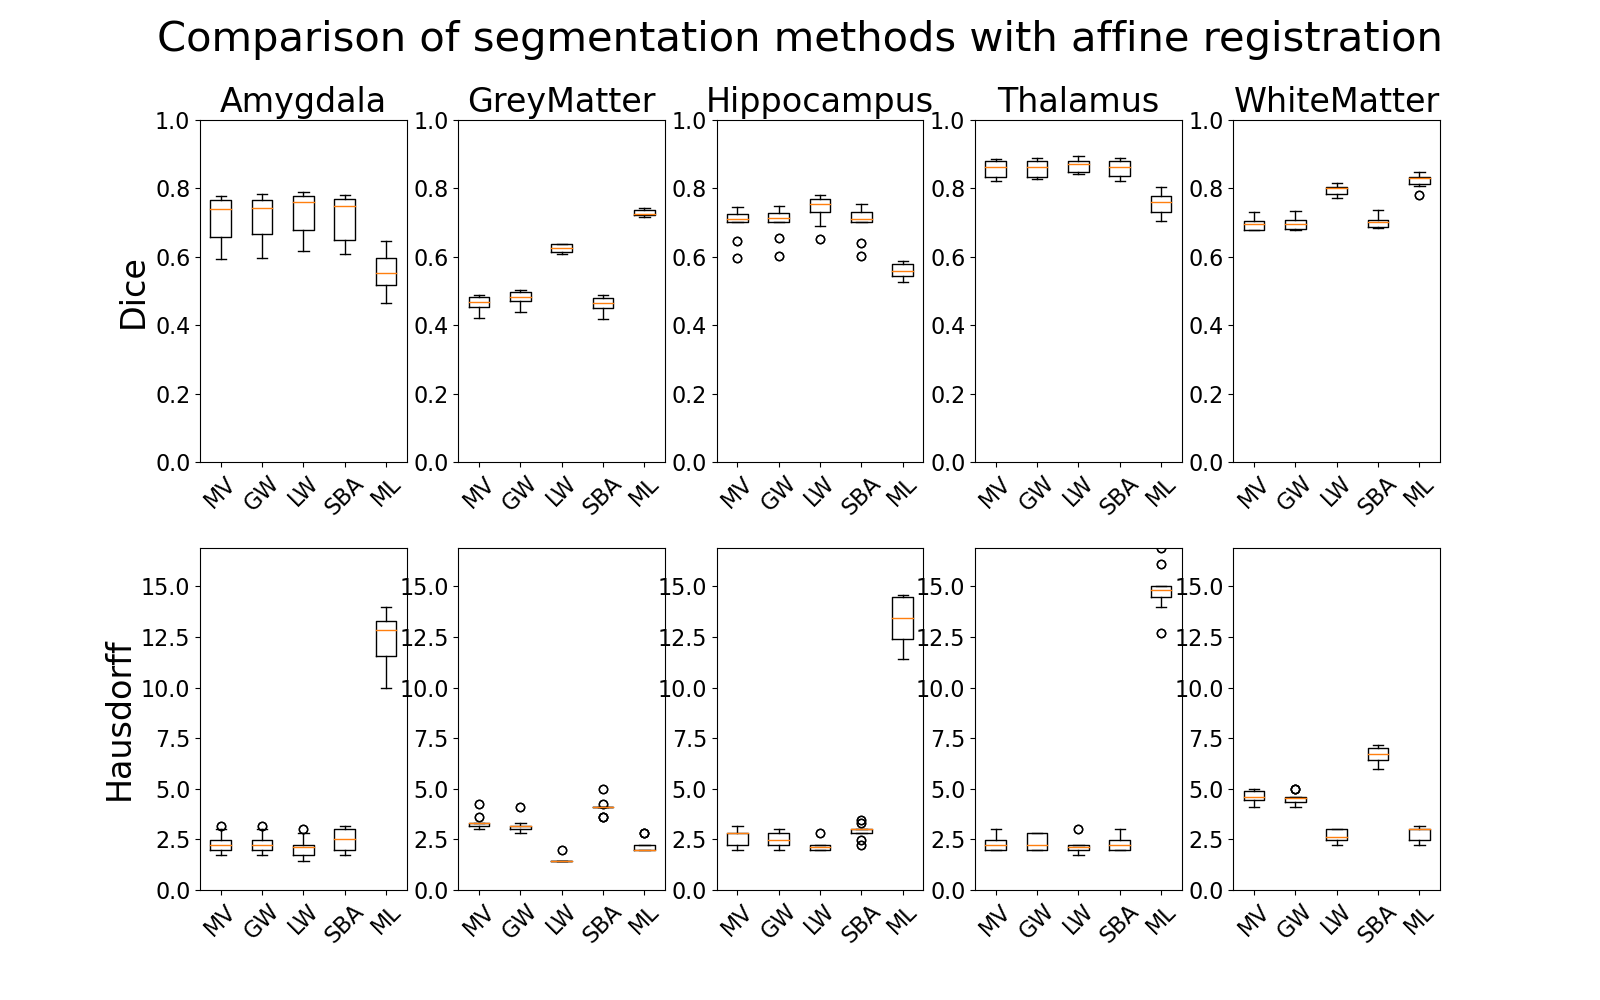
\includegraphics[width = .48 \textwidth]{img/boxplot_Affine_all}
	\caption{Dice and Hausdorff distance result for majority voting (MV), global weighted (GW), local weighted (LW), shape based averaging (SBA) and machine learning (ML) segmentations preceded by affine registration}
	\label{fig:boxplotAff}
\end{figure}

For the smaller parts of the brain (Amygdala, Hippocampus and Thalamus), all atlas-based segmentation methods have similar results. Machine learning has more difficulties with those brain parts. On the other hand, it gives better results with grey and white matter. Local weighted atlas significantly performs better than any other atlas-based segmentation methods for those brain parts. It is the best overall segmentation methods.

The same segmentation methods with non-rigid registration are represented in figure \ref{fig:boxplotNR}.

\begin{figure}[h!]
	\centering
	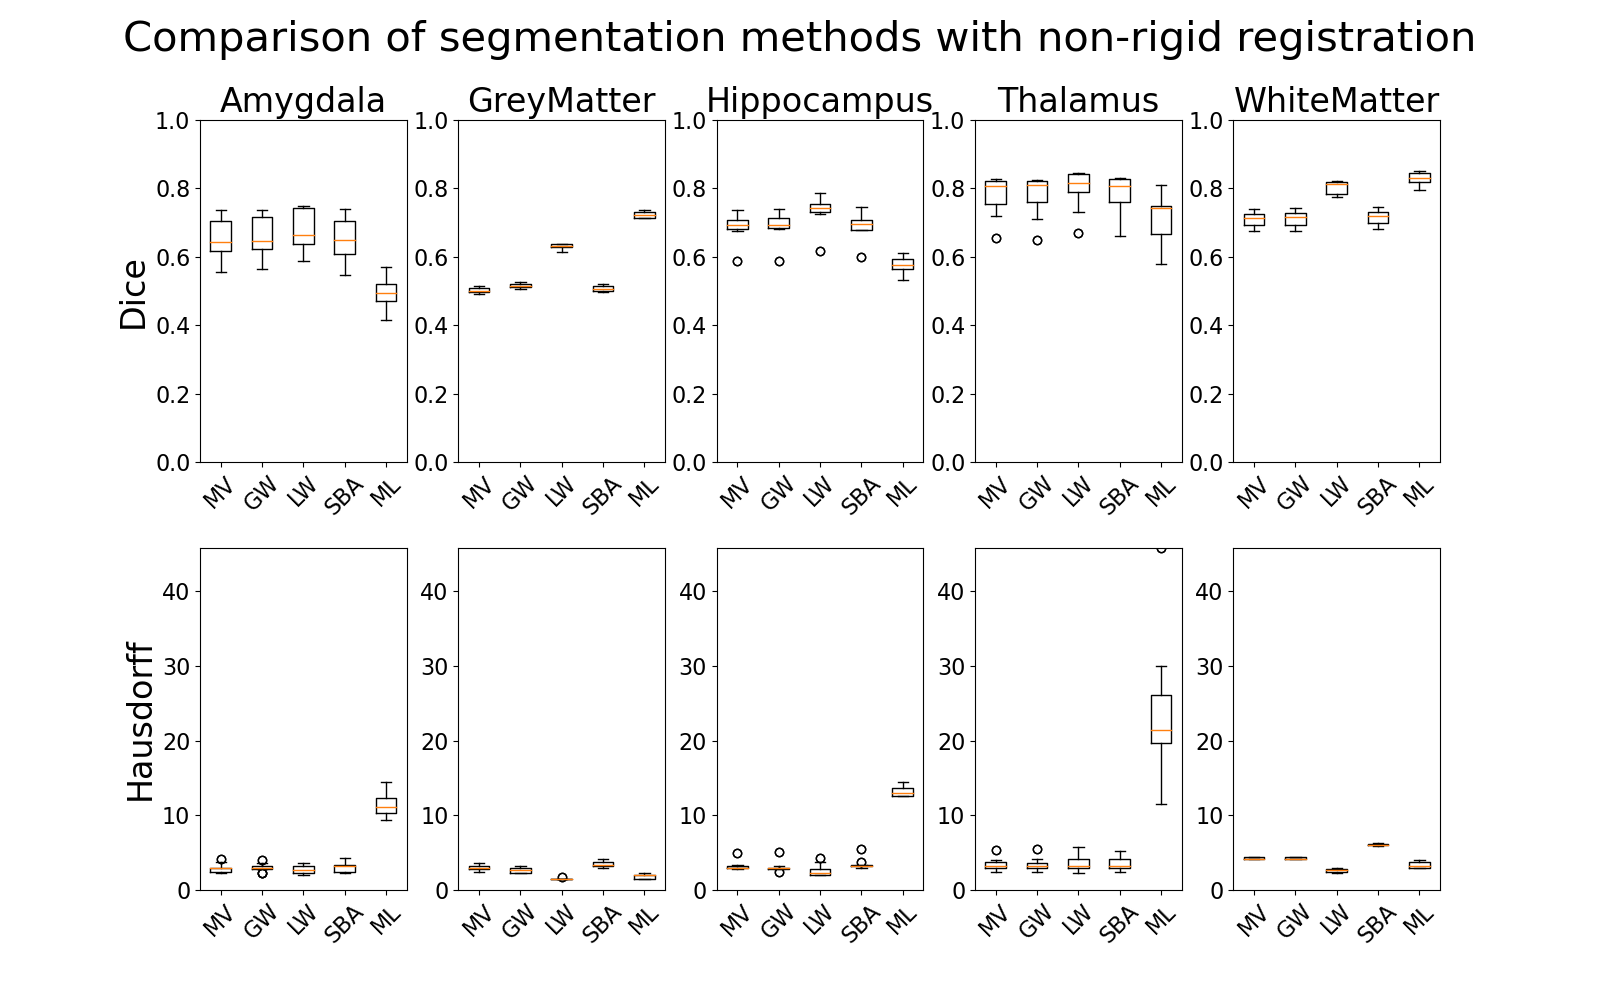
\includegraphics[width = .48 \textwidth]{img/boxplot_NR_all}
	\caption{Dice and Hausdorff distance result for majority voting (MV), global weighted (GW), local weighted (LW), shape based averaging (SBA) and machine learning (ML) segmentations preceded by non-rigid registration}
	\label{fig:boxplotNR}
\end{figure}

In general, the results are very similar to the one with affine registration. Machine learning seems to struggle even more with the Thalamus, as the Hausdorff distance suggests.
